\documentclass[11pt]{article}
\usepackage{amsmath,amssymb,geometry,enumitem,array,tikz,fancyhdr}
\geometry{margin=0.8in}
\setlength{\parindent}{0pt}
\setlength{\parskip}{0.45em}
\setlist[itemize]{leftmargin=*,itemsep=0.25em,topsep=0.2em}
\setlist[enumerate]{leftmargin=*,itemsep=0.5em,topsep=0.3em}
\pagestyle{fancy}
\fancyhf{}
\fancyhead[L]{\small Calculus BC: Integration \& Differential Equations}
\fancyfoot[C]{\thepage}
\setlength{\headheight}{14pt}
\newcommand{\topic}[2]{\clearpage\section*{#1 --- #2}}
\newcommand{\practice}[2]{\clearpage\section*{#1 --- 30-Minute Practice}\textbf{#2} Show your setup and reasoning. Use exact values unless directed otherwise. The time beside each problem is a pacing target, not a separate deadline.}
\newcommand{\continued}[1]{\clearpage\section*{#1 --- Practice, continued}}
\newcommand{\mins}[1]{\hfill\textit{(#1 min)}}
\newcommand{\dx}{\,dx}
\begin{document}
\begin{center}
{\LARGE\bfseries Calculus BC Study Guide}\\[0.4em]
{\Large Integration \& Differential Equations}\\[0.7em]
{\large Seven focused lessons + seven 30-minute practice sets}
\end{center}

\section*{How to use this packet}
\begin{enumerate}
\item Study one topic at a time. Read the formal statement, then explain in your own words what it lets you do.
\item Cover the worked example and try it yourself. Compare each step, not just the final answer. This study time is \textbf{not} part of the 30 minutes.
\item Set a \textbf{30-minute timer} for that topic's two-page practice set. There are six problems per set; their suggested times total 30 minutes. Unless a set says otherwise, close the guide and work without a calculator.
\item If stuck, write a valid setup and move on. After the timer, use the separate worked-solutions packet. Correct the first incorrect step, then retry the problem without looking.
\end{enumerate}
Practice time is \textbf{210 minutes total}, best split across seven sessions. Thirty minutes is a planning target; learning speed varies. Use extra paper if needed.

\section*{Topic map}
\begingroup
\renewcommand{\arraystretch}{1.35}
\begin{tabular}{@{}p{0.10\linewidth}p{0.75\linewidth}@{}}
6.1 & Indefinite integral rules and initial conditions\\
6.2 & LRAM, RRAM, MRAM; definite-integral properties; integral MVT\\
6.3 & Inscribed/circumscribed rectangles and their infinite limits\\
6.4 & Fundamental Theorem of Calculus (FTC)\\
6.6 & Rectangle, trapezoidal, Simpson approximations; error estimates\\
7.1 & Slope fields and Euler's method\\
7.2 & Antiderivatives using $u$-substitution
\end{tabular}
\endgroup

\section*{Scope and references}
The numbering above follows your class list, \textbf{not College Board's topic numbering}. Here, ``infinite rectangles'' means the limit of finite lower/upper rectangle sums, not an improper integral over an infinite interval.

\textbf{AP alignment.} College Board's \emph{AP Calculus AB and BC Course and Exam Description}, Topics 6.2--6.9, 7.3--7.5, and 8.1, covers the related integration, slope-field, Euler, and average-value skills. Euler's method is BC-only. Simpson's rule and derivative-based quadrature error bounds are included as \textbf{classroom extensions}, not listed AP requirements. They are different from BC series error bounds.

\textbf{Mathematical reference.} OpenStax, \emph{Calculus Volume 2}, Section 3.6, ``Numerical Integration,'' for midpoint/trapezoidal/Simpson formulas and error bounds. Examples and practice problems here are original. Test tips are mathematical safeguards, not a promise of a particular scoring rubric.

\topic{6.1}{Indefinite Integral Rules}
\subsection*{Formal statement / idea}
An \textbf{antiderivative} of $f$ on an interval is a function $F$ satisfying $F'(x)=f(x)$ throughout that interval. If $F$ is one antiderivative, then all are $F+C$:
\[
\int f(x)\dx=F(x)+C.
\]
This is a \emph{family of functions}, not a number or an area. Linearity gives
$\int[af(x)+bg(x)]\dx=a\int f(x)\dx+b\int g(x)\dx$ for constants $a,b$.

\begin{center}
\renewcommand{\arraystretch}{1.2}
\begin{tabular}{ll}
\textbf{Integrand} & \textbf{Antiderivative (add $C$)}\\ \hline
$x^p$, $p\ne-1$ & $x^{p+1}/(p+1)$\\
$1/x$ & $\ln|x|$ on an interval avoiding $0$\\
$e^x$; $a^x$ ($a>0$, $a\ne1$) & $e^x$; $a^x/\ln a$\\
$\cos x$; $\sin x$ & $\sin x$; $-\cos x$\\
$\sec^2x$; $\csc^2x$ & $\tan x$; $-\cot x$\\
$\sec x\tan x$; $\csc x\cot x$ & $\sec x$; $-\csc x$\\
$1/(1+x^2)$; $1/\sqrt{1-x^2}$ & $\arctan x$; $\arcsin x$ ($|x|<1$)
\end{tabular}
\end{center}
Use each rule only where the integrand is defined. For a linear input, if $F'=f$ and $k\ne0$,
$\int f(kx+b)\dx=F(kx+b)/k+C$.

\subsection*{Why it is used}
Integration reverses differentiation: recover position from velocity, or a quantity from its rate. An initial condition selects one member of the family.

\subsection*{Classic worked example}
Find $F$ if $F'(x)=6x^2-4/x+3\cos x$, $x>0$, and $F(1)=5$.
\[
F(x)=2x^3-4\ln x+3\sin x+C.
\]
Insert the \emph{function value}: $5=2+3\sin1+C$, so $C=3-3\sin1$.
Differentiate the result to check: $6x^2-4/x+3\cos x$ is recovered.

\subsection*{Test gotchas}
\begin{itemize}
\item Rewrite roots/reciprocals as powers first. The power rule fails at $p=-1$.
\item $\int\sin x\dx=-\cos x+C$; the minus sign is easy to lose.
\item Do not integrate a product by multiplying antiderivatives. Linearity applies to \emph{sums}, not products or quotients.
\item Indefinite integrals need $+C$; initial conditions determine it. Definite-integral values do not need $+C$.
\end{itemize}

\practice{6.1}{No calculator.}
\begin{enumerate}
\item Evaluate both integrals. \mins{4}
\[
\text{(a) }\int(8x^3-6x+5)\dx\qquad
\text{(b) }\int\left(3\sqrt{x}-\frac{2}{x^2}\right)\dx,\quad x>0.
\]
\vfill
\item Evaluate both integrals on intervals where they are defined. \mins{5}
\[
\text{(a) }\int\left(\frac4x+2e^x\right)\dx\qquad
\text{(b) }\int\left(3\sec^2x-2\sin x+\frac{1}{1+x^2}\right)\dx.
\]
\vfill
\item Evaluate both integrals. \mins{4}
\[
\text{(a) }\int6\cos(3x)\dx\qquad
\text{(b) }\int5e^{-2x}\dx.
\]
\vfill
\end{enumerate}
\continued{6.1}
\begin{enumerate}[start=4]
\item Find $F(x)$ if $F'(x)=3x^2-4x+2$ and $F(1)=5$. Verify your result by differentiation and substitution. \mins{5}
\vfill
\item A student writes
\[
\int\left(\frac1x+\cos x\right)\dx=\frac{\ln|x|}{x}+\sin x.
\]
Differentiate the proposed answer, identify the errors, and give a correct general antiderivative. \mins{6}
\vfill
\item A particle has velocity $v(t)=6t-4$ meters per second and position $s(0)=7$ meters.
Find $s(t)$, its position at $t=3$, and its displacement from $t=0$ to $t=3$. Explain why the last two answers differ. \mins{6}
\vfill
\end{enumerate}

\topic{6.2}{Riemann Sums and Definite Integrals}
\subsection*{Formal statement / idea}
For a partition $a=x_0<x_1<\cdots<x_n=b$, write $\Delta x_i=x_i-x_{i-1}$ and choose $x_i^*\in[x_{i-1},x_i]$. A Riemann sum is
\[
\sum_{i=1}^n f(x_i^*)\Delta x_i.
\]
If $f$ is continuous on $[a,b]$, these sums approach the same number as the largest interval width tends to zero. That number is $\int_a^b f(x)\dx$.

For $n$ equal intervals, $\Delta x=(b-a)/n$ and $x_i=a+i\Delta x$:
\begin{align*}
L_n&=\Delta x\sum_{i=1}^n f(x_{i-1}) &&\text{LRAM: left endpoint},\\
R_n&=\Delta x\sum_{i=1}^n f(x_i) &&\text{RRAM: right endpoint},\\
M_n&=\Delta x\sum_{i=1}^n f\left(\frac{x_{i-1}+x_i}{2}\right)
&&\text{MRAM: midpoint}.
\end{align*}
\textbf{Plain language:} width $\times$ height, added across every interval. For unequal widths, multiply \emph{each} height by its own width.

\subsection*{Why it is used}
A rate table may be all you have. Rectangle sums estimate the accumulated change even without an antiderivative. Rate units times input units give total-change units.

\subsection*{Classic worked example}
For $f(x)=x^2+1$ on $[0,2]$ with $n=2$, $\Delta x=1$:
\[
\begin{array}{c|cc|c}
&[0,1]&[1,2]&\text{sum}\\ \hline
\text{Left heights}&f(0)=1&f(1)=2&L_2=3\\
\text{Right heights}&f(1)=2&f(2)=5&R_2=7\\
\text{Midpoint heights}&f(1/2)=5/4&f(3/2)=13/4&M_2=9/2
\end{array}
\]
Because $f$ increases, $L_2\le\int_0^2f\le R_2$. The midpoint height is $f(\text{midpoint})$, \textbf{not} the average of endpoint heights.

\subsection*{Test gotchas}
\begin{itemize}
\item $n$ intervals need $n+1$ endpoints but only $n$ rectangle heights.
\item Increasing: left under, right over. Decreasing: reverse. Without monotonicity, endpoint labels alone do not determine the error direction.
\item A definite integral is \emph{signed} accumulation. Geometric area uses $|f|$.
\item A table of endpoints does not supply midpoint values unless those inputs are also listed. Do not invent them by averaging outputs.
\end{itemize}

\topic{6.2}{Properties, Average Value, and Integral MVT}
\subsection*{Formal statements}
For integrable $f,g$ and constants $\alpha,\beta$:
\begin{align*}
\int_a^a f\dx&=0,& \int_b^a f\dx&=-\int_a^b f\dx,\\
\int_a^c f\dx+\int_c^b f\dx&=\int_a^b f\dx,&
\int_a^b(\alpha f+\beta g)\dx&=\alpha\int_a^b f\dx+\beta\int_a^b g\dx.
\end{align*}
For $a<b$, if $f\le g$ then $\int_a^b f\le\int_a^b g$. In particular,
if $m\le f(x)\le M$, then $m(b-a)\le\int_a^b f\le M(b-a)$.

If $f$ is even, $\int_{-a}^a f=2\int_0^a f$; if $f$ is odd, $\int_{-a}^a f=0$ (assuming integrability).

\textbf{Average value:} for integrable $f$ on $[a,b]$, $a<b$,
\[
f_{\mathrm{avg}}=\frac{1}{b-a}\int_a^b f(x)\dx.
\]
\textbf{Mean Value Theorem for Integrals:} if $f$ is \emph{continuous} on $[a,b]$, $a<b$, there exists $c\in(a,b)$ such that
\[
f(c)=f_{\mathrm{avg}},\qquad\text{equivalently}\qquad
\int_a^b f(x)\dx=f(c)(b-a).
\]
\subsection*{Why it is used}
Properties combine known integrals without re-integrating. Average value is the constant height giving the same signed area. Continuity guarantees that the function actually attains that average height somewhere in the interval.

\subsection*{Classic worked examples}
If $\int_0^2 f=5$ and $\int_2^5 f=-1$, then
\[
\int_0^5 f=4,\qquad \int_5^0 f=-4,\qquad
\int_0^5(2f+3)\dx=2(4)+3(5)=23.
\]
For $f(x)=x^2$ on $[0,3]$, $\int_0^3x^2\dx=9$. Thus
$f_{\mathrm{avg}}=9/3=3$. Since $x^2$ is continuous, the theorem applies.
Solve $c^2=3$: only $c=\sqrt3$ lies in $(0,3)$.

\subsection*{Test gotchas}
\begin{itemize}
\item Average \emph{function value} is $\int f/(b-a)$, not $(f(b)-f(a))/(b-a)$, which is average rate of change.
\item The integral MVT uses $f(c)$, not $f'(c)$. State continuity when invoking it.
\item Average the function over the interval, not merely its two endpoint values.
\item $\int_a^b k\dx=k(b-a)$: integrating a constant still introduces interval length.
\end{itemize}

\practice{6.2}{No calculator.}
\begin{enumerate}
\item For $f(x)=x^2$ on $[0,2]$, compute $L_2$, $R_2$, and $M_2$. List the sample inputs used for each sum. \mins{6}
\vfill
\item Water enters a tank at a continuous, increasing rate $r(t)$ liters/minute.
\[
\begin{array}{c|rrrr}t\text{ (min)}&0&2&5&6\\\hline r(t)&1&3&4&5\end{array}
\]
Using the three listed subintervals, estimate the amount entering with left and right sums. State which is a lower estimate, and include units. \mins{5}
\vfill
\item Suppose $\int_0^2 f\dx=3$, $\int_2^5 f\dx=-4$, and $\int_0^5g\dx=6$.
Find (a) $\int_0^5 f\dx$, (b) $\int_5^2 f\dx$, and (c) $\int_0^5(2f-g+1)\dx$. \mins{4}
\vfill
\end{enumerate}
\continued{6.2}
\begin{enumerate}[start=4]
\item Find the average value of $f(x)=x^2+1$ on $[0,3]$ and all $c\in(0,3)$ satisfying the integral MVT conclusion. State why the theorem applies. You may use $\int_0^3(x^2+1)\dx=12$. \mins{5}
\vfill
\item The graph of $f$ forms a triangle above the $x$-axis on $[0,2]$ with base $2$ and height $3$. On $[2,4]$ it forms a semicircle below the axis with radius $1$.
Find (a) $\int_0^4 f\dx$, (b) $\int_0^4|f|\dx$, and (c) the average value of $f$ on $[0,4]$. \mins{5}
\vfill
\item Let $f(x)=0$ for $0\le x<1$ and $f(x)=2$ for $1\le x\le2$.
Find its average value on $[0,2]$. Is there a $c\in(0,2)$ where $f(c)$ equals that average? Does this contradict the integral MVT? Explain. \mins{5}
\vfill
\end{enumerate}

\topic{6.3}{Inscribed and Circumscribed Rectangles}
\subsection*{Formal statement / idea}
Let $f$ be continuous on $[a,b]$ and $P$ a partition. On each subinterval set
\[
m_i=\min_{[x_{i-1},x_i]}f,\quad M_i=\max_{[x_{i-1},x_i]}f,\quad
\ell(P)=\sum_i m_i\Delta x_i,\quad U(P)=\sum_i M_i\Delta x_i.
\]
Then $\ell(P)\le\int_a^b f\dx\le U(P)$. If $f\ge0$, these are the areas of \textbf{inscribed} and \textbf{circumscribed} rectangles. For signed $f$, call them lower/upper sums instead of ordinary rectangle areas.

As the largest subinterval width $\|P\|$ tends to $0$,
\[
\boxed{\lim_{\|P\|\to0}\ell(P)=\int_a^b f(x)\dx
=\lim_{\|P\|\to0}U(P).}
\]
A continuous function is integrable, so the upper/lower gap tends to zero.

\subsection*{Why it is used}
This makes ``area under a curve'' precise and traps the exact value between computable bounds. The infinite process is a \emph{limit}; you never add literal rectangles of width zero.

\subsection*{Classic geometric example}
For $f(x)=x^2$ on $[0,1]$, increasing behavior means lower rectangles use left endpoints, and upper rectangles use right endpoints.
\begin{center}
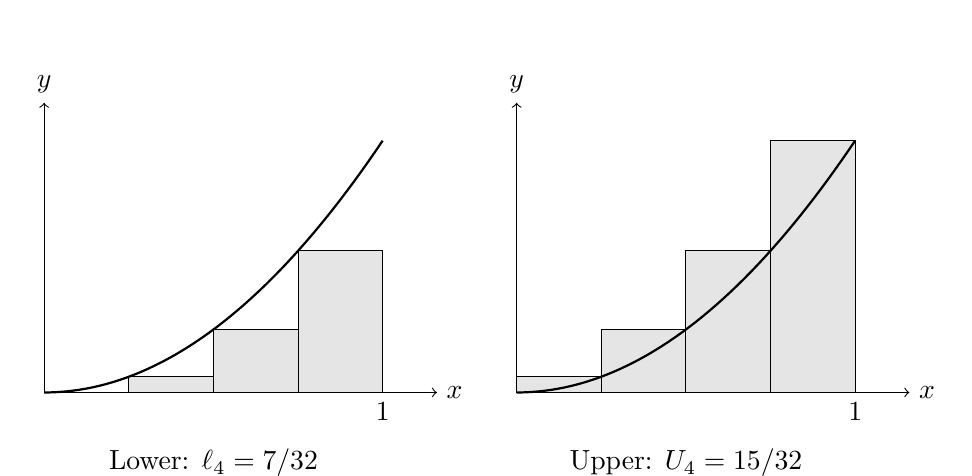
\begin{tikzpicture}[x=4.3cm,y=3.2cm]
\foreach \i in {0,1,2,3}{
\pgfmathsetmacro{\a}{\i/4}\pgfmathsetmacro{\b}{(\i+1)/4}
\pgfmathsetmacro{\h}{\a*\a}
\draw[fill=gray!20] (\a,0) rectangle (\b,\h);}
\draw[->] (0,0)--(1.16,0) node[right]{$x$};
\draw[->] (0,0)--(0,1.15) node[above]{$y$};
\draw[thick,domain=0:1,samples=50] plot (\x,{\x*\x});
\node[below] at (1,0){$1$};\node at (0.5,-0.28){Lower: $\ell_4=7/32$};
\begin{scope}[xshift=6cm]
\foreach \i in {0,1,2,3}{
\pgfmathsetmacro{\a}{\i/4}\pgfmathsetmacro{\b}{(\i+1)/4}
\pgfmathsetmacro{\h}{\b*\b}
\draw[fill=gray!20] (\a,0) rectangle (\b,\h);}
\draw[->] (0,0)--(1.16,0) node[right]{$x$};
\draw[->] (0,0)--(0,1.15) node[above]{$y$};
\draw[thick,domain=0:1,samples=50] plot (\x,{\x*\x});
\node[below] at (1,0){$1$};\node at (0.5,-0.28){Upper: $U_4=15/32$};
\end{scope}
\end{tikzpicture}
\end{center}
\subsection*{Test gotchas}
\begin{itemize}
\item ``Inscribed'' does not always mean left. For decreasing $f\ge0$, right endpoints give the inscribed rectangles.
\item If a curve turns within an interval, its maximum/minimum may be inside, not at an endpoint.
\item Merely saying $n\to\infty$ is not enough for arbitrary partitions: the \emph{largest width} must tend to zero. Equal partitions satisfy this automatically.
\end{itemize}

\topic{6.3}{Turning a Rectangle Sum into an Exact Integral}
\subsection*{Classic limit calculation}
Continue with $f(x)=x^2$ on $[0,1]$ and $n$ equal intervals.
Then $\Delta x=1/n$, left inputs are $(i-1)/n$, and right inputs are $i/n$.
\begin{align*}
\ell_n&=\frac1n\sum_{i=1}^n\left(\frac{i-1}{n}\right)^2
=\frac{(n-1)n(2n-1)}{6n^3}
=\frac13-\frac{1}{2n}+\frac{1}{6n^2},\\
U_n&=\frac1n\sum_{i=1}^n\left(\frac{i}{n}\right)^2
=\frac{n(n+1)(2n+1)}{6n^3}
=\frac13+\frac{1}{2n}+\frac{1}{6n^2}.
\end{align*}
Both limits are $1/3$. Since $\ell_n\le\int_0^1x^2\dx\le U_n$, the squeeze theorem gives $\int_0^1x^2\dx=1/3$. Notice $U_n-\ell_n=1/n\to0$.

\subsection*{Recognizing a limit of sums}
For continuous $f$,
\[
\int_a^b f(x)\dx=
\lim_{n\to\infty}\sum_{i=1}^n
f\left(a+i\frac{b-a}{n}\right)\frac{b-a}{n}.
\]
Read the expression in this order:
\begin{enumerate}
\item Identify the rectangle width $\Delta x=(b-a)/n$.
\item Identify the sample input $x_i=a+i\Delta x$.
\item Identify the function applied to that input.
\end{enumerate}
For example,
\[
\lim_{n\to\infty}\sum_{i=1}^n
\sqrt{1+\left(2+\frac{3i}{n}\right)^2}\frac3n
=\int_2^5\sqrt{1+x^2}\dx.
\]
No evaluation is needed to translate the sum.

\subsection*{Useful finite-sum identities}
\[
\sum_{i=1}^n1=n,\qquad
\sum_{i=1}^n i=\frac{n(n+1)}2,\qquad
\sum_{i=1}^n i^2=\frac{n(n+1)(2n+1)}6.
\]
These simplify \emph{finite} sums before taking the limit. Keep the width factor outside the sum all the way through.

\subsection*{Test gotchas}
\begin{itemize}
\item The starting point $a$ may be nonzero. A width of $3/n$ tells you the interval length is $3$, not that the interval is $[0,3]$.
\item One rectangle sum is usually an approximation; the limit is the exact integral.
\item When translating, keep the integrand and width together. A missing $1/n$ changes the problem completely.
\end{itemize}

\practice{6.3}{No calculator. You may use the finite-sum identities on the preceding page.}
\begin{enumerate}
\item For $f(x)=4-x$ on $[0,4]$, use four equal subintervals. Draw the inscribed rectangles, compute their total area, and compute the circumscribed total. Identify which endpoint rule produces each. \mins{5}
\vfill
\item For $f(x)=x^2$ on $[0,2]$, write $\ell_n$ and $U_n$ as sigma sums with $n$ equal intervals. Simplify both expressions in terms of $n$ using the finite-sum identities. \mins{7}
\vfill
\item Take the limits of your two expressions from Problem 2 and state the exact area under $x^2$ on $[0,2]$. Explain why the two limits determine the area. \mins{3}
\vfill
\end{enumerate}
\continued{6.3}
\begin{enumerate}[start=4]
\item Write each limit as a definite integral; do not evaluate. \mins{5}
\[
\text{(a) }\lim_{n\to\infty}\sum_{i=1}^n\left[1+\left(2+\frac{3i}{n}\right)^2\right]\frac3n
\qquad
\text{(b) }\lim_{n\to\infty}\sum_{i=1}^n\cos\left(\frac{\pi i}{2n}\right)\frac{\pi}{2n}.
\]
\vfill
\item Write $\int_1^4\sqrt{x+2}\dx$ as a limit of right-endpoint sums using $n$ equal subintervals. State $\Delta x$ and $x_i$ separately. \mins{4}
\vfill
\item Let $f(x)=4-(x-2)^2$ on $[0,4]$, using the partition $0,1,3,4$.
Find the lower and upper sums. Is either the left sum or the right sum an upper sum for this partition? Justify by identifying the extrema on $[1,3]$. \mins{6}
\vfill
\end{enumerate}

\topic{6.4}{Fundamental Theorem of Calculus}
\subsection*{Formal statements}
\textbf{Accumulation form.} If $f$ is continuous on an interval containing $a$, then
$A(x)=\int_a^x f(t)\,dt$ is differentiable at interior points and $A'(x)=f(x)$.
With differentiable bounds and continuous $f$ on the relevant interval,
\[
\frac{d}{dx}\int_{u(x)}^{v(x)}f(t)\,dt
=f(v(x))v'(x)-f(u(x))u'(x).
\]
\textbf{Evaluation form.} If $f$ is continuous on $[a,b]$ and $F'=f$, then
\[
\int_a^b f(x)\dx=F(b)-F(a).
\]
\subsection*{Why it is used}
The FTC links accumulation to rate: differentiate accumulated change to recover the rate; integrate a rate to recover net change. It also replaces long limit-of-sums calculations with endpoint evaluation.

\subsection*{Classic worked examples}
For $G(x)=\int_1^{x^2}\sqrt{1+t^4}\,dt$, no elementary antiderivative is needed:
\[
G'(x)=\sqrt{1+(x^2)^4}\,(2x)=2x\sqrt{1+x^8}.
\]
The outer FTC step supplies the integrand at the upper bound; the chain rule supplies $2x$.

For an evaluation,
\[
\int_0^2(3x^2-4x)\dx=[x^3-2x^2]_0^2=0.
\]
Zero is \emph{net} signed area, not zero total area: this integrand changes sign.

If $H(x)=\int_0^x(t-2)\,dt$, then $H'=x-2$ and $H''=1$.
Thus $H$ decreases for $x<2$, increases for $x>2$, and has a local minimum at $2$.

\subsection*{Test gotchas}
\begin{itemize}
\item Differentiate an accumulation integral by substituting into the integrand, not by differentiating that integrand. $A'=f$, while $A''=f'$ when $f'$ exists.
\item Moving upper bound: multiply by its derivative. Moving lower bound: also subtract that term.
\item To find where $A$ increases, inspect the \emph{sign of $f$}, not whether $f$ increases. For concavity of $A$, inspect $f'$.
\item In $\int f(t)\,dt$, $t$ is a dummy variable. The simple moving-bound formula assumes the integrand has no other dependence on $x$.
\item A discontinuity inside an interval can invalidate direct use of the stated evaluation theorem. Do not blindly apply it across a vertical asymptote.
\end{itemize}

\practice{6.4}{No calculator.}
\begin{enumerate}
\item Evaluate both integrals. \mins{4}
\[
\text{(a) }\int_0^2(3x^2-2x+1)\dx\qquad
\text{(b) }\int_1^e\frac1x\dx.
\]
\vfill
\item Let $A(x)=\int_2^x\sqrt{1+t^3}\,dt$ for $x>0$.
Find $A'(x)$, $A'(2)$, and $A''(x)$. \mins{4}
\vfill
\item Differentiate both functions. \mins{5}
\[
\text{(a) }G(x)=\int_0^{x^3}\cos(t^2)\,dt\qquad
\text{(b) }H(x)=\int_x^4\ln(1+t^2)\,dt.
\]
\vfill
\end{enumerate}
\continued{6.4}
\begin{enumerate}[start=4]
\item Let $K(x)=\int_{x^2}^{3x}(1+t^2)\,dt$. Find $K'(x)$ and $K'(1)$. \mins{5}
\vfill
\item Let $F(x)=\int_0^x(t^2-4)\,dt$ for $-3\le x\le3$.
Find the open intervals where $F$ increases and decreases, the locations of its interior local extrema, and the intervals where it is concave up and down. Justify with derivatives. \mins{7}
\vfill
\item An object's rate of change of mass is $m'(t)=2t-3$ grams/minute for $0\le t\le4$, and $m(0)=10$ grams.
Find its net mass change, its mass at $t=4$, and the time when its mass is smallest on this interval. \mins{5}
\vfill
\end{enumerate}

\topic{6.6}{Numerical Integration}
\subsection*{Formal rules}
Write $I=\int_a^b f(x)\dx$, $h=(b-a)/n$, and $f_i=f(a+ih)$ for equal subintervals.
Rectangle rules $L_n,R_n,M_n$ are defined in 6.2. The composite trapezoidal rule is
\[
T_n=\frac h2[f_0+2f_1+\cdots+2f_{n-1}+f_n]
=\frac{L_n+R_n}{2}.
\]
For \textbf{unequal widths}, use
$T=\sum_{i=1}^n\frac{x_i-x_{i-1}}2[f(x_{i-1})+f(x_i)]$.

\textbf{Simpson's rule (classroom extension):} equal widths and \emph{even} $n$ are required:
\[
S_n=\frac h3\left[f_0+
4\sum_{\substack{i=1\\i\text{ odd}}}^{n-1}f_i+
2\sum_{\substack{i=2\\i\text{ even}}}^{n-2}f_i+f_n\right].
\]
The weights are $1,4,2,4,2,\ldots,4,1$; for $n=2$ they are $1,4,1$.
For continuous $f$, these composite rules converge to $I$ as $h\to0$ (even $n$ for Simpson).

\subsection*{Why it is used}
Numerical rules approximate integrals from data or when a usable antiderivative is unavailable. Rectangles use constant heights; trapezoids use straight-line tops; Simpson's rule uses quadratic pieces.

\subsection*{Classic worked example}
Approximate $\int_0^2x^3\dx$ using $n=2$, so $h=1$, and values $0,1,8$:
\[
T_2=\frac12[0+2(1)+8]=5,\qquad
S_2=\frac13[0+4(1)+8]=4.
\]
The exact integral is $4$. Simpson is exact for polynomials of degree at most three; it is \emph{not} always exact for other functions.

\subsection*{Error direction}
\begin{center}
\begin{tabular}{c|cc}
\textbf{Behavior throughout $[a,b]$}&\textbf{Underestimate}&\textbf{Overestimate}\\\hline
$f'\ge0$&$L_n$&$R_n$\\
$f'\le0$&$R_n$&$L_n$\\
$f''\ge0$&$M_n$&$T_n$\\
$f''\le0$&$T_n$&$M_n$
\end{tabular}
\end{center}
Equality can occur. Monotonicity controls left/right errors; concavity controls midpoint/trapezoidal errors. Concavity alone does not determine Simpson's error sign.

\subsection*{Test gotchas}
Count intervals, not table entries. Do not use equal-width formulas on uneven data. Simpson needs an even number of intervals, not an even number of data values. Show the weighted sum before entering arithmetic into a calculator.

\topic{6.6}{Error Estimates and Guaranteed Accuracy}
\subsection*{Formal bounds (classroom extension)}
Let $a<b$, use equal widths, and write $E_Q=|I-Q_n|$ for \textbf{absolute error}. Assume the indicated derivatives are continuous on $[a,b]$, and that $K_j$ is an upper bound for $|f^{(j)}(x)|$ on the \emph{whole} interval.
\[
\begin{array}{c|c|c}
\text{Rule}&\text{Derivative needed}&\text{Guaranteed upper bound}\\\hline
L_n\text{ or }R_n&|f'|\le K_1&E_L,E_R\le\dfrac{K_1(b-a)^2}{2n}\\[0.8em]
M_n&|f''|\le K_2&E_M\le\dfrac{K_2(b-a)^3}{24n^2}\\[0.8em]
T_n&|f''|\le K_2&E_T\le\dfrac{K_2(b-a)^3}{12n^2}\\[0.8em]
S_n\ (n\text{ even})&|f^{(4)}|\le K_4&E_S\le\dfrac{K_4(b-a)^5}{180n^4}
\end{array}
\]
\textbf{Why these are useful:} the exact integral may be unknown, yet a derivative bound still guarantees accuracy. A bound $E_Q\le B$ places $I$ inside $[Q_n-B,Q_n+B]$. It does \emph{not} say the actual error equals $B$.

\subsection*{Classic worked example: choose the number of intervals}
For $I=\int_0^2x^2\dx$, $f''=2$, so take $K_2=2$. To guarantee trapezoidal error at most $0.01$,
\[
\frac{2(2)^3}{12n^2}=\frac4{3n^2}\le\frac1{100}
\quad\Longrightarrow\quad n^2\ge\frac{400}{3}.
\]
Since $11^2<400/3<12^2$, choose $n=12$. With $n=2$, the bound is $1/3$; indeed $T_2=3$ and $I=8/3$, so the actual error is $1/3$ in this example.

For the rectangle bound, on one width-$h$ interval, the derivative bound gives
$|f(x)-f(x_{i-1})|\le K_1(x-x_{i-1})$. Integrate to get error at most $K_1h^2/2$; adding $n$ such bounds yields $K_1(b-a)^2/(2n)$.

\subsection*{Test gotchas}
\begin{itemize}
\item Bound the \emph{absolute value} of the derivative everywhere, not just its value at a convenient endpoint. A larger valid bound is safe but less efficient.
\item Solve the inequality, then round $n$ \emph{up}. For Simpson, round up again if necessary to make $n$ even. For a strict tolerance $E<\varepsilon$, ensure the bound is strictly below it.
\item Doubling $n$ divides these bounds by $2$, $4$, $4$, and $16$, respectively; this is a statement about the bounds, not an exact prediction of every actual error.
\item If $I\ne0$, relative error is $|I-Q_n|/|I|$; percent error is $100$ times that. Neither is the same as absolute error.
\end{itemize}

\practice{6.6}{Calculator allowed for arithmetic only. You may use the rule and error-bound formulas.}
\begin{enumerate}
\item For $\int_0^2x^2\dx$, compute $L_2,R_2,M_2,T_2,S_2$.
Compare each with the exact value $8/3$ and state whether it is low, high, or exact. \mins{7}
\vfill
\item A rate $r(t)$ in liters/minute is recorded below. Use trapezoids on the listed intervals to approximate $\int_0^6r(t)\,dt$, including units. \mins{3}
\[
\begin{array}{c|rrrr}t&0&1&3&6\\\hline r(t)&2&4&3&5\end{array}
\]
\vfill
\item A twice-differentiable function satisfies $f'(x)<0$ and $f''(x)>0$ throughout $[a,b]$.
Classify $L_n$, $R_n$, $M_n$, and $T_n$ as underestimates or overestimates. Explain which condition controls each pair. \mins{3}
\vfill
\end{enumerate}
\continued{6.6}
\begin{enumerate}[start=4]
\item For $f(x)=x^4$ on $[0,1]$, find valid bounds $K_1,K_2,K_4$.
Use $n=4$ to find absolute-error bounds for left/right rectangles, midpoint, trapezoidal, and Simpson's rule. \mins{6}
\vfill
\item For a smooth function on $[0,2]$, suppose $|f''|\le3$ and $|f^{(4)}|\le10$.
Find the smallest allowed $n$ certified by the respective formulas to guarantee error at most $0.001$ for (a) the trapezoidal rule and (b) Simpson's rule. \mins{6}
\vfill
\item A numerical estimate is $Q=2.4$ with a guaranteed absolute-error bound $0.03$.
(a) Give an interval guaranteed to contain the exact integral.
(b) A later exact calculation gives $I=2.38$. Find the actual absolute error and percent error (round percent to three decimal places).
(c) A student says $|I-Q|=0.03$ must hold. Explain the mistake. \mins{5}
\vfill
\end{enumerate}

\topic{7.1}{Slope Fields}
\subsection*{Formal statement / idea}
For a first-order differential equation
\[
\frac{dy}{dx}=F(x,y),
\]
a \textbf{slope field} places a short line segment of slope $F(x_0,y_0)$ at each selected point $(x_0,y_0)$. A solution curve satisfies $y'(x)=F(x,y(x))$ at every point and is tangent to those local directions. An initial condition specifies a point the desired solution must pass through.

\textbf{Equilibrium:} $y(x)=k$ is a constant solution if $F(x,k)=0$ for \emph{every} $x$ under consideration. A single horizontal segment does not establish an equilibrium.

\subsection*{Why it is used}
A field shows solution behavior without solving the equation: where solutions rise or fall, where they level off, and how an initial value selects a path.

\subsection*{Classic worked example}
For $y'=y-x$, the slopes at $(0,1),(1,1),(1,0)$ are $1,0,-1$.
Every point on $y=x$ has slope zero, but $y=x$ is \emph{not} a solution: that curve's derivative is $1$, not $0$.
\begin{center}
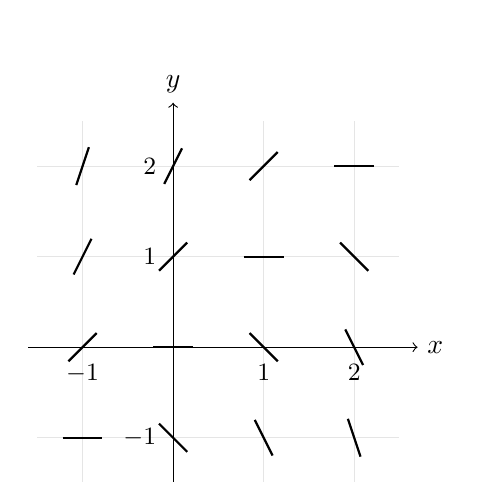
\begin{tikzpicture}[scale=1.15]
\draw[step=1,gray!20] (-1.5,-1.5) grid (2.5,2.5);
\draw[->] (-1.6,0)--(2.7,0) node[right]{$x$};
\draw[->] (0,-1.6)--(0,2.7) node[above]{$y$};
\foreach \x in {-1,0,1,2}{\foreach \y in {-1,0,1,2}{
\pgfmathsetmacro{\m}{\y-\x}
\pgfmathsetmacro{\d}{0.22/sqrt(1+\m*\m)}
\draw[thick] ({\x-\d},{\y-\m*\d})--({\x+\d},{\y+\m*\d});}}
\foreach \x in {-1,1,2}{\node[below] at (\x,-0.08){\small $\x$};}
\foreach \y in {-1,1,2}{\node[left] at (-0.08,\y){\small $\y$};}
\end{tikzpicture}
\end{center}
\subsection*{Test gotchas}
\begin{itemize}
\item Substitute \emph{both} coordinates. The output is a slope, not a new $y$-coordinate.
\item If $F$ depends only on $x$, slopes repeat vertically. If only on $y$, they repeat horizontally.
\item A solution must follow the field smoothly, not connect the centers of all its segments.
\item For uniqueness, a standard sufficient hypothesis is that $F$ and $\partial F/\partial y$ are continuous near the initial point. Under it, solution curves cannot cross there. Do not claim noncrossing without appropriate hypotheses.
\end{itemize}

\topic{7.1}{Euler's Method}
\subsection*{Formal rule}
Given $y'=F(x,y)$ and $y(x_0)=y_0$, choose step size $h$ and set
\[
\boxed{x_{k+1}=x_k+h,\qquad y_{k+1}=y_k+hF(x_k,y_k).}
\]
This is a numerical approximation, based on the tangent-line model
$y(x+h)\approx y(x)+h\,y'(x)$.

\subsection*{Why it is used}
Euler follows the slope field one short tangent step at a time to estimate a solution value without finding an exact solution formula.

\subsection*{Classic worked example}
For $y'=x+y$, $y(0)=1$, estimate $y(0.5)$ using two equal steps. Here $h=(0.5-0)/2=0.25$.
\[
\begin{array}{c|c|c|c|c}
k&x_k&y_k&F(x_k,y_k)&y_{k+1}=y_k+hF(x_k,y_k)\\\hline
0&0&1&1&1.25\\
1&0.25&1.25&1.5&1.625
\end{array}
\]
Thus $y(0.5)\approx1.625$. The second slope uses the \emph{updated} point $(0.25,1.25)$, not the initial $y$ again.

\subsection*{Concavity and error}
A tangent line lies below a concave-up solution and above a concave-down solution. This determines the error direction of a \emph{single tangent step from an exact point}. For multiple Euler steps, justify propagation of the error for the given equation; a slope field sketch alone is not a universal error proof.

For $y'=y$, $y(0)=1$, forward Euler uses $y_{k+1}=(1+h)y_k$.
The exact solution is $e^x$. For $h>0$, $1+h<e^h$, so $(1+h)^k<e^{kh}$: this particular forward-Euler sequence underestimates the solution.

\subsection*{Test gotchas}
\begin{itemize}
\item New value $=$ old value $+$ step size $\times$ current slope. A slope by itself is not the next value.
\item Recompute the slope at every new $(x_k,y_k)$. Show a table so the updates are visible.
\item To move left, $h$ is negative. Count updates, not rows: two steps require three solution points.
\item Keep unrounded values during the iteration. Round only the requested final approximation.
\item If $y'=F(x,y)$, then along a solution $y''=F_x+F_y\,y'$. Substitute the differential equation when studying concavity.
\end{itemize}

\practice{7.1}{Calculator allowed for arithmetic only. Use exact fractions or terminating decimals; do not round intermediate values.}
\begin{enumerate}
\item For $y'=x+y$, draw a slope field at all nine points with $x,y\in\{-1,0,1\}$. Then sketch a short solution curve through $(0,0)$. State its slope at $(0,0)$ and whether that solution is constant. \mins{6}
\begin{center}
\begin{tikzpicture}[scale=1.0]
\draw[step=1,gray!25] (-1.5,-1.5) grid (1.5,1.5);
\draw[->] (-1.6,0)--(1.7,0) node[right]{$x$};
\draw[->] (0,-1.6)--(0,1.7) node[above]{$y$};
\foreach \x in {-1,0,1}{\foreach \y in {-1,0,1}{\fill (\x,\y) circle (1pt);}}
\foreach \x in {-1,1}{\node[below] at (\x,-0.05){$\x$};}
\foreach \y in {-1,1}{\node[left] at (-0.05,\y){$\y$};}
\end{tikzpicture}
\end{center}
\item A field has equal slopes along each horizontal row. Its segments are horizontal at $y=2$, positive below $y=2$, and negative above $y=2$.
Which equation matches: $y'=x$, $y'=2-y$, or $y'=y-2$? Justify, and identify an equilibrium solution. \mins{3}
\vfill
\item Given $y'=x+y$, $y(0)=1$, use two Euler steps of size $0.5$ to estimate $y(1)$. Show the current point, slope, and update for each step. \mins{6}
\vfill
\end{enumerate}
\continued{7.1}
\begin{enumerate}[start=4]
\item Given $y'=x-y$, $y(1)=2$, use two equal Euler steps to estimate $y(0)$. Show the signed step size and both updates. \mins{5}
\vfill
\item Given $y'=2-y$, $y(0)=0$:
(a) use three Euler steps of size $0.5$ to estimate $y(1.5)$;
(b) derive $y''$ in terms of $y$ and determine the solution's concavity while $y<2$. \mins{5}
\vfill
\item Given $y'=y$, $y(0)=1$:
(a) estimate $y(1)$ with one Euler step of size $1$;
(b) repeat with two steps of size $0.5$;
(c) given the exact solution $y=e^x$, compare both estimates with $e\approx2.71828$ and decide which is closer. \mins{5}
\vfill
\end{enumerate}

\topic{7.2}{Antiderivatives by $u$-Substitution}
\subsection*{Formal statement / idea}
Suppose $g$ is continuously differentiable and $f$ is continuous on an interval containing the values of $g$. If $F'=f$, the reverse chain rule gives
\[
\int f(g(x))g'(x)\dx=F(g(x))+C.
\]
Write $u=g(x)$ and $du=g'(x)\,dx$ to expose the basic integral.
For definite integrals,
\[
\int_a^b f(g(x))g'(x)\dx=\int_{g(a)}^{g(b)}f(u)\,du.
\]
For this substitution identity, $g$ need not be increasing; the transformed limits carry the direction.

\subsection*{Why it is used}
A complicated expression may really be a basic antiderivative with an inside function. Substitution works when its derivative appears, possibly multiplied by a constant.

\subsection*{Classic worked examples}
For $\int x(x^2+4)^3\dx$, choose $u=x^2+4$. Then $du=2x\,dx$, so $x\,dx=du/2$:
\[
\int x(x^2+4)^3\dx=\frac12\int u^3\,du
=\frac{u^4}{8}+C=\frac{(x^2+4)^4}{8}+C.
\]
Check: differentiating yields $(1/8)\cdot4(x^2+4)^3\cdot2x=x(x^2+4)^3$.

For $\int_0^1\frac{2x}{1+x^2}\dx$, use $u=1+x^2$, $du=2x\,dx$.
The limits become $u(0)=1$, $u(1)=2$, so
\[
\int_1^2\frac1u\,du=[\ln u]_1^2=\ln2.
\]
This is the pattern $\int g'(x)/g(x)\dx=\ln|g(x)|+C$ on an interval where $g\ne0$.

\subsection*{Test gotchas}
\begin{itemize}
\item Write $du$ before integrating. Supply a missing \emph{constant} factor correctly; do not invent a missing variable factor.
\item In a rewritten $u$-integral, every $x$ must be eliminated. An $x$ left over signals unfinished substitution.
\item For an indefinite integral, return to $x$ and add $C$. For a definite integral, either change the limits to $u$ or return to $x$ before using the original limits. Never mix them.
\item $\int\cos(x^2)\dx$ is not handled by simply writing $\sin(x^2)/(2x)$: the derivative factor $2x$ is absent. Not every integral is a direct substitution problem.
\end{itemize}

\practice{7.2}{No calculator. Show the substitution and differential in each applicable problem.}
\begin{enumerate}
\item Evaluate both integrals. \mins{5}
\[
\text{(a) }\int 2x(x^2+5)^4\dx\qquad
\text{(b) }\int3\cos(3x+1)\dx.
\]
\vfill
\item Evaluate both integrals. \mins{5}
\[
\text{(a) }\int\frac{x}{x^2+9}\dx\qquad
\text{(b) }\int\frac{e^x}{1+e^x}\dx.
\]
\vfill
\item Evaluate both integrals. \mins{5}
\[
\text{(a) }\int\frac{\sin x}{\sqrt{2+\cos x}}\dx\qquad
\text{(b) }\int\frac{6x}{1+9x^4}\dx.
\]
\vfill
\end{enumerate}
\continued{7.2}
\begin{enumerate}[start=4]
\item Evaluate $\int_0^2x\sqrt{x^2+5}\dx$ using transformed limits. \mins{5}
\vfill
\item Find $F(x)$ if $F'(x)=2x e^{x^2}$ and $F(0)=3$. Verify both the derivative and the initial condition. \mins{4}
\vfill
\item A student claims $\int\cos(x^2)\dx=\sin(x^2)/(2x)+C$ for $x\ne0$.
(a) Differentiate the proposed antiderivative to test the claim.
(b) Explain why $u=x^2$ does not turn this integrand directly into $\int\cos u\,du$.
(c) Evaluate the related integral $\int x\cos(x^2)\dx$. \mins{6}
\vfill
\end{enumerate}
\end{document}
